\input templates/header

\usepackage{epigraph}
\usepackage[normalem]{ulem}
\usepackage{xcolor}
\usepackage{colortbl}
\usepackage{tikz}
\usepackage[normalem]{ulem}
\usepackage[absolute,overlay]{textpos}
\usetikzlibrary{trees}
\usetikzlibrary{shapes}
\usetikzlibrary{positioning}

\setlength{\epigraphwidth}{6cm}

\renewcommand*{\arraystretch}{1.2}
\usepackage{xmpmulti}
\usepackage{listings}

\lstset{
  basicstyle=\ttfamily,
%  columns=fullflexible,
  keywordstyle=\color{red}\bfseries,
  commentstyle=\color{blue},
  showstringspaces=false,
  escapeinside={<@}{@>},
}

\newcommand*\circled[1]{\tikz[baseline=(char.base)]{
      \node[circle,ball color=blue, shade, 
 color=white,inner sep=1.2pt] (char) {\tiny #1};}}


\title[ASD - Programmazione Dinamica]{\textbf{Algoritmi e Strutture Dati}\\[24pt]Programmazione dinamica -- Parte 3}

\graphicspath{{figs/13/}}

\begin{document}



%-------------------------------------------------------------------------
\FrameTitle{}

%-------------------------------------------------------------------------
\FrameContent

%%%%%%%%%%%%%%%%%%%%%%%%%%%%%%%%%%%%%%%%%%%%%%%%%%%%%%%%%%%%%%%%%%%%%%%%%%%%%
\section{String matching approssimato}
%%%%%%%%%%%%%%%%%%%%%%%%%%%%%%%%%%%%%%%%%%%%%%%%%%%%%%%%%%%%%%%%%%%%%%%%%%%%%

%-------------------------------------------------------------------------
\begin{frame}{String matching approssimato}

\vspace{-9pt}
\begin{myboxtitle}[Definizione]

Un'\alert{occorrenza $k$-approssimata} di $P$ in $T$, dove
\BI
\item $P = p_1 \ldots p_m$ è una stringa detta \alert{pattern}
\item $T = t_1 \ldots t_n$ è una stringa detta \alert{testo}, con $m \leq n$,
\EI
è una copia di $P$ in $T$ in cui sono ammessi $k$ "errori" (o differenze) tra caratteri di $P$ e caratteri di $T$, del seguente tipo:
\begin{enumerate}
\item i corrispondenti caratteri in $P, T$ sono diversi (\alert{sostituzione}) 
\item un carattere in $P$ non è incluso in $T$ (\alert{inserimento})
\item un carattere in $T$ non è incluso in $P$ (\alert{cancellazione})
\end{enumerate}
\end{myboxtitle}

\begin{myboxtitle}[Problema -- Approximated string matching]
Trovare un'occorrenza $k$-approssimata di $P$ in $T$ con $k$ minimo\\ 
($0 \leq k \leq m$).
\end{myboxtitle}

\end{frame}

%-------------------------------------------------------------------------
\begin{frame}{Esempio}

\vspace{-9pt}
\begin{myboxtitle}[Esempio]
T = \texttt{questoèunoscempio} \\
P = \texttt{unesempio}
\end{myboxtitle}

\begin{myboxtitle}[Domande]
\BIL
\item Qual è il minimo valore $k$ per cui si trova una occorrenza $k$-approssimata di $P$ in $T$?
\item A partire da dove?
\item Con quali errori?
\EIL
\end{myboxtitle}

\end{frame}

%-------------------------------------------------------------------------
\begin{frame}{Sottostruttura ottima}

\vspace{-9pt}
\begin{myboxtitle}[Definizione]
Sia $DP[0 \ldots m, 0 \ldots n]$ una tabella di programmazione dinamica
tale che $DP[i][j]$ contiene il minimo valore $k$ per cui esiste un'occorrenza $k$-approssimata di $P(i)$ in $T(j)$, che termina nella posizione $j$.
\end{myboxtitle}

\BB{Quattro possibilità}
\smallskip
\begin{tabular}{ll}
$DP[i-1][j-1]$, se $p_i = t_j$ &	avanza su entrambi i caratteri (uguali) \\
$DP[i-1][j-1]+1$, se $p_i \neq t_j$ &	avanza su entrambi i caratteri  (\alert{sost.}) \\
$DP[i-1][j]+1$				& avanza sul pattern (\alert{inserimento})\\
$DP[i][j-1]+1$				& avanza sul testo (\alert{cancellazione})\\
\end{tabular}

\end{frame}

%-------------------------------------------------------------------------
\begin{frame}{Sottostruttura ottima}

\vspace{-9pt}
\[
DP[i][j] = \begin{cases}
0  & \textrm{$i=0$}\\
i  & \textrm{$j=0$}\\
\min\{ DP[i-1][j-1] + \delta, & \delta = \IIF(p_i=t_j,0,1)\\
\qquad\, DP[i-1][j] + 1,\\ 
\qquad\, DP[i][j-1] + 1\} & \textrm{altrimenti}
\end{cases}
\]

\begin{center}
\IG{0.4}{stringmatching.pdf}
\end{center}

\end{frame}

%-------------------------------------------------------------------------
\begin{frame}{Ricostruzione della soluzione finale}

\vspace{-9pt}
\BIL
\item $DP[m][j] = k$ se e solo se esiste un'occorrenza $k$-approssimata di $P$ in $T(j)$ che
termina nella posizione $j$.
\item La soluzione del problema è data dal più piccolo valore $DP[m][j]$, per $0 \leq j \leq n$
\EIL

\begin{center}
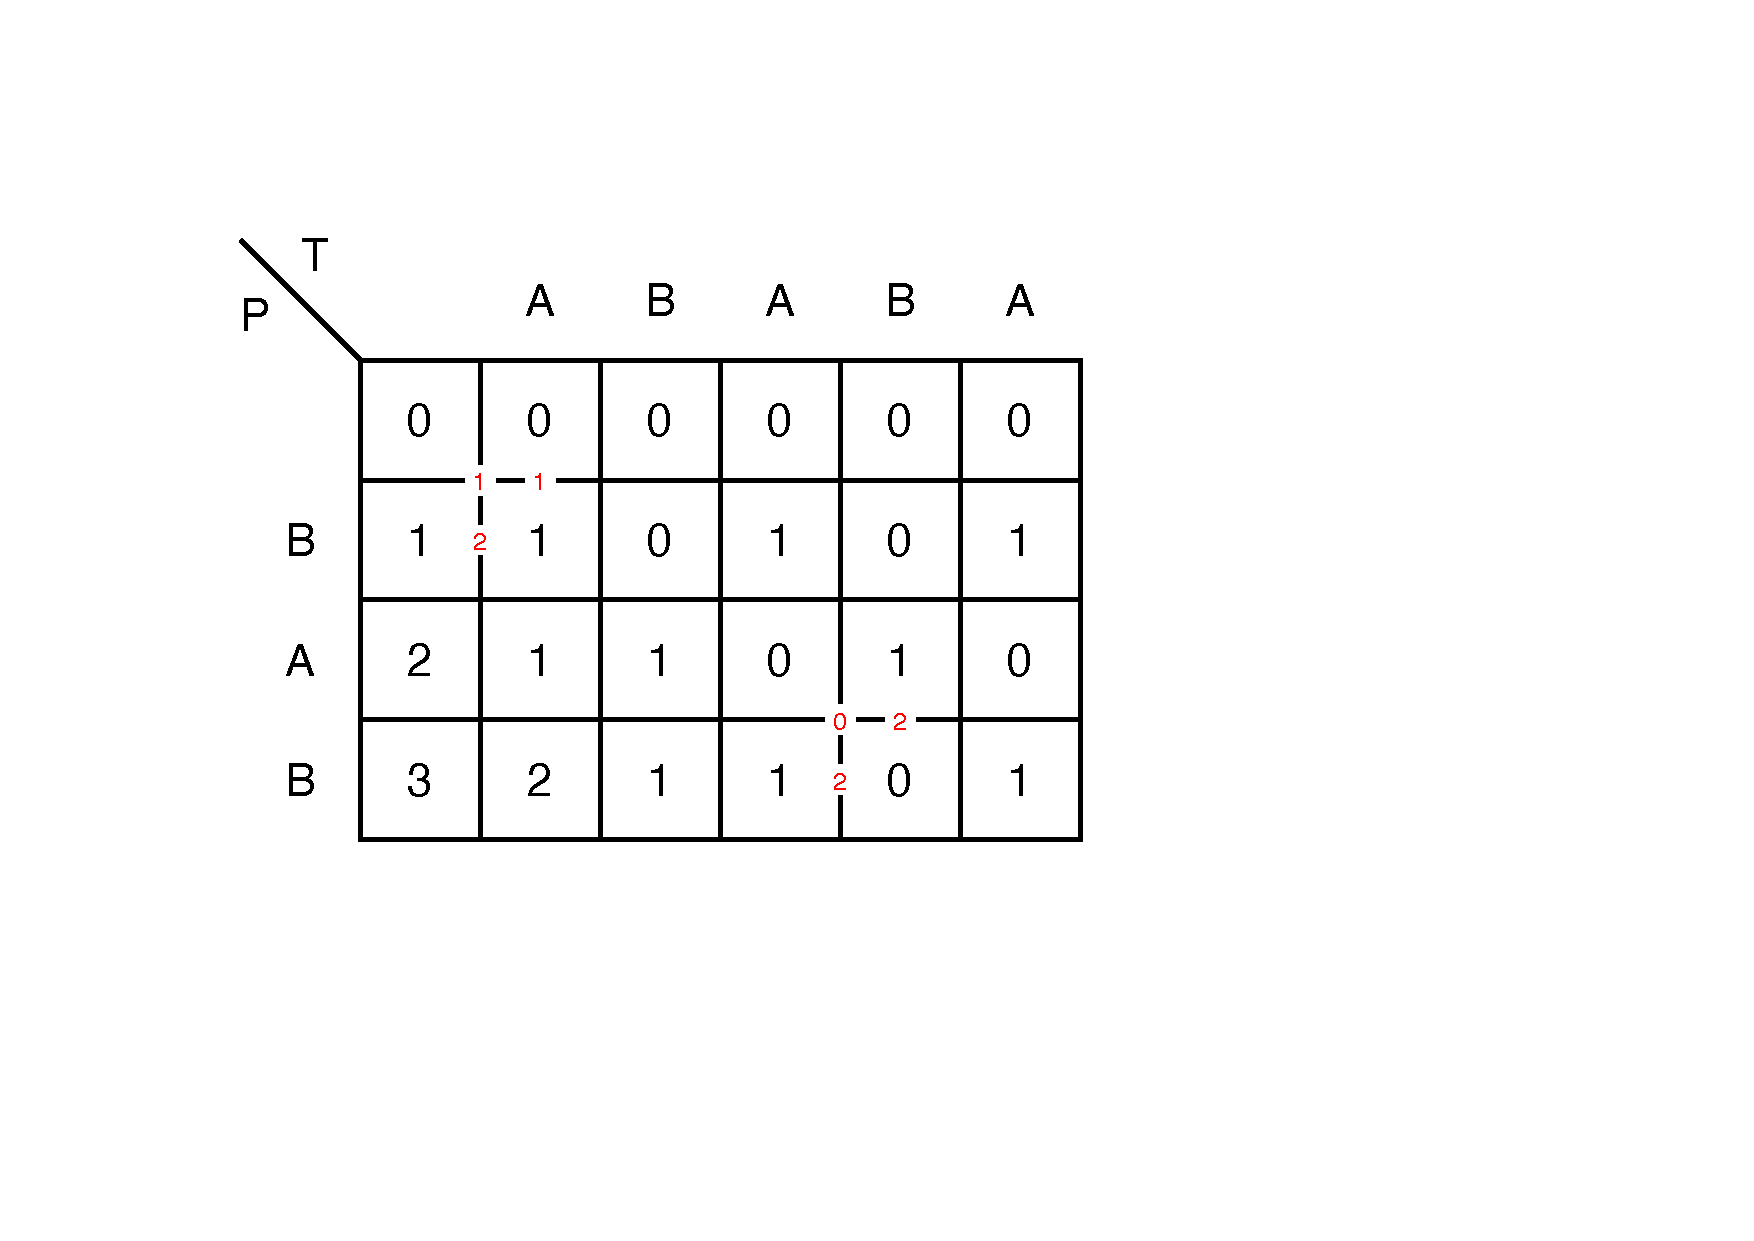
\includegraphics[width=0.5\textwidth]{stringmatching2.pdf}
\end{center}

\end{frame}

%-------------------------------------------------------------------------
\begin{frame}[shrink=3]{}

\vspace{-9pt}
\begin{Procedure}
\caption[A]{\INTEGER\ \stringmatching($\Item[\,]\ P,\ \Item[\,]\ T,\ \INTEGER\ m,\ \INTEGER\ n$)}

$\INTARRAY[\,]\ DP = \NEW\ \INTEGER[0 \mldots m][ 0 \mldots n]$\;
\lFor(\Comment*[f]{Base case: $i=0$}){$j = 0$ \TO\ $n$}{$DP[0][j] = 0$}
\lFor(\Comment*[f]{Base case: $j=0$}){$i = 1$ \TO\ $m$}{$DP[i][0] = i$}
\For(\Comment*[f]{General case}){$i = 1$ \TO\ $m$}{
  \For{$j = 1$ \TO\ $n$}{
    $DP[i][j] = DP[i-1][j-1] + \IIF(P[i] = T[j], 0, 1)$\;
    $DP[i][j] = \MIN(DP[i][j], DP[i-1][j]+1)$\;
    $DP[i][j] = \MIN(DP[i][j], DP[i][j-1]+1)$\;
  }
}
\INTEGER\ $\Min = DP[m,0]$\Comment*{Compute min last row}
\INTEGER\ $\Pos = 0$\;
\For{$j = 1$ \TO\ $n$}{
  \If{$DP[m][j] < \Min$}{
  $\Min = DP[m][j]$\;
  $\Pos = j$\;
  }
}
\Return $\Pos$\;
\end{Procedure}

\end{frame}

%-------------------------------------------------------------------------
\begin{frame}{String matching approssimato}

\vspace{-9pt}
\begin{myboxtitle}[Take-home message -- prendi e porta a casa]
Non è detto che "la soluzione finale" si trovi nella casella "in basso a destra"; è invece possibile che la soluzione debba essere ricercata essa 
stessa nella tabella $DP$
\end{myboxtitle}

\end{frame}

%-------------------------------------------------------------------------
\begin{frame}{Reality check}

\vspace{-9pt}
\BB{
Approximate String Matching è un esempio di \alert{string metric}:

\begingroup
\small
\begin{quote}
[...] \alert{is a metric that measures distance ("inverse similarity") between two strings} [...]

String metrics are used heavily in information integration and are currently used in areas including fraud detection, fingerprint analysis, plagiarism detection, ontology merging, DNA analysis, RNA analysis, image analysis, evidence-based machine learning, database data deduplication, data mining, incremental search, data integration, and semantic knowledge integration.
\end{quote}
\endgroup

\url{https://en.wikipedia.org/wiki/String_metric}
}

\begin{myboxtitle}[Esempi]
\alert{Edit distance}, detta anche \alert{distanza di Levenshtein}
\end{myboxtitle}

\end{frame}


%%%%%%%%%%%%%%%%%%%%%%%%%%%%%%%%%%%%%%%%%%%%%%%%%%%%%%%%%%%%%%%%%%%%%%%%%%%%%
\section{Prodotto di catena di matrici}
%%%%%%%%%%%%%%%%%%%%%%%%%%%%%%%%%%%%%%%%%%%%%%%%%%%%%%%%%%%%%%%%%%%%%%%%%%%%%


%-------------------------------------------------------------------------
\begin{frame}{Prodotto di catena di matrici}

\vspace{-9pt}
\begin{myboxtitle}[Problema]
Data una sequenza di $n$ matrici $A_1, A_2, A_3, \ldots, A_n$, compatibili due a due al prodotto, vogliamo calcolare il loro prodotto.
\BIL
\item  Il prodotto di matrici non è \alert{commutativo} \ldots .
\item  \ldots .ma è \alert{associativo}: $(A_1 \cdot A_2) \cdot A_3 = A_1 \cdot (A_2 \cdot A_3)$ 
\EIL
\end{myboxtitle}

\BB{Cosa vogliamo ottimizzare}
\BIL
\item Il prodotto di matrici si basa sulla \alert{moltiplicazione scalare} come operazione elementare
\item Vogliamo calcolare il prodotto delle $n$ matrici impiegando il più basso numero possibile di moltiplicazioni scalari
\EIL

\end{frame}

%-------------------------------------------------------------------------
\begin{frame}{Esempio 1}
    
\vspace{-9pt}
\begin{columns}[T]
\column{0.20\textwidth}
\begingroup
\setlength\arrayrulewidth{1pt}
\begin{tabular}{|c|c|}
\hline
A & $100 \times 1$ \\\hline
B & $1 \times 100$ \\\hline
C & $100 \times 1$ \\\hline
\end{tabular}    
\endgroup
\column{0.75\textwidth}
\vspace{-16pt}    
\IG{1.0}{matrici-esempio1.pdf}
\end{columns}

\end{frame}

%-------------------------------------------------------------------------
\begin{frame}{Esempio 2}

\vspace{-9pt}
\begin{columns}[T]
\column{0.20\textwidth}
\begingroup
\setlength\arrayrulewidth{1pt}
\begin{tabular}{|c|c|}
\hline
A & $50 \times 10$ \\\hline
B & $10 \times 40$ \\\hline
C & $40 \times 30$ \\\hline
D & $30 \times 5$ \\\hline
\end{tabular}    
\endgroup
\column{0.75\textwidth}
\vspace{-16pt}    
\IG{1.0}{matrici-esempio2.pdf}
\end{columns}

\end{frame}


%-------------------------------------------------------------------------
\begin{frame}{Parentesizzazione}

\vspace{-9pt}
\begin{myboxtitle}[Parentesizzazione]
Una \alert{parentesizzazione} $P_{i,j}$ del prodotto $A_i \cdot A_{i+1} \cdot \cdot \cdot A_j$ consiste:
\BI
\item nella matrice $A_i$, se $i = j$; 
\item nel prodotto di due parentesizzazioni ($P_{i,k} \cdot P_{k+1,j}$), altrimenti.
\EI
\end{myboxtitle}

\begin{columns}[T]
\column{0.42\textwidth}
\BB{Esempio}
\[
(A_1 \cdot (A_2 \cdot A_3 ))  \alert{\times}  (A_4 \cdot (A_5 \cdot A_6 )) 
\]
In questo caso, $k=3$ e il prodotto evidenziato 
è detto "\alert{ultimo prodotto}"
\column{0.50\textwidth}
\vspace{-6pt}
\IG{1.0}{esempio-par.pdf}
\end{columns}

\end{frame}

%-------------------------------------------------------------------------
\begin{frame}{Parentesizzazione ottima}

\vspace{-9pt}
\begin{myboxtitle}[Parentesizzazione ottima]
La parentesizzazione che richiede il minor numero di moltiplicazioni scalari per essere completata, fra tutte le parentesizzazioni possibili.
\end{myboxtitle}

\begin{myboxtitle}[Motivazione]
Vale la pena preprocessare i dati per cercare la parentesizzazione migliore, per risparmiare tempo dopo nel calcolo vero e proprio
\end{myboxtitle}

\begin{myboxtitle}[Domanda]
Quante sono le parentesizzazioni possibili?
\begin{center}
\begin{tabular}{|c|r|r|r|r|r|r|r|r|r|r|}
\hline
$n$ & \phantom{0}1 & \phantom{0}2 & \phantom{0}3 & \phantom{0}4 & \phantom{0}5 & \phantom{0}6 & \phantom{0}7 & \phantom{0}8 & \phantom{0}9 & \phantom{0}10 \\\hline
$P(n)$ & 1 & 1 & 2 & 5 & ? & ? & ? & ? & ? & ? \\\hline
\end{tabular}
\end{center}
\end{myboxtitle}
\end{frame}

%-------------------------------------------------------------------------
\begin{frame}{Parentesizzazione ottima}

\vspace{-9pt}
\BIL
\item $P(n)$: numero di parentesizzazioni per $n$ matrici $A_1 \cdot \ldots \cdot A_n$
\item L'ultimo prodotto può occorrere in $n-1$ posizioni diverse
\item Fissato l'indice $k$ dell'ultimo prodotto, abbiamo:
\BI
\item $P(k)$ parentesizzazioni per $A_1 \cdot \ldots \cdot A_k$
\item $P(n-k)$ parentesizzazioni per $A_{k+1} \cdot \ldots \cdot A_n$
\EI
\EIL

\[
  P(n) = \begin{cases}
    1 & n = 1 \\
    \sum_{i=1}^{n-1} P(k)P(n-k) & n>1
    \end{cases}
\]

\smallskip
\begin{center}
\begin{tabular}{|c|r|r|r|r|r|r|r|r|r|r|}
\hline
$n$ & \phantom{0}1 & \phantom{0}2 & \phantom{0}3 & \phantom{0}4 & \phantom{0}5 & \phantom{0}6 & \phantom{0}7 & \phantom{0}8 & \phantom{0}9 & \phantom{0}10 \\\hline
$P(n)$ & 1 & 1 & 2 & 5 & 14 & 42 & 132 & 429 & 1430 & 4862 \\\hline
\end{tabular}
\end{center}
\end{frame}

%-------------------------------------------------------------------------
\begin{frame}{Parentesizzazione ottima}

\vspace{-9pt}
\begin{myboxtitle}[Numero di Catalan]
\[
P(n+1) = C(n) = \frac{1}{n+1} {2n\choose n} = \frac{(2n)!}{(n+1)!n!} = \Omega\left(\frac{4^n}{n^{3/2}}\right)
\]
\end{myboxtitle}

\begin{columns}[T]
\column{0.48\textwidth}
\BB{In matematica}
$C(n)$: numero di modi in cui un poligono convesso con $n+2$ lati può essere suddiviso in triangoli.
\IG{0.8}{catalan-hexagon.png}
\column{0.48\textwidth}
\BB{Esercizio}
Dimostrare che $P(n) = \Omega(2^n)$

\BB{Implicazione}
Algoritmi di forza bruta non vanno quindi bene
\end{columns}

\end{frame}

%-------------------------------------------------------------------------
\begin{frame}{Definizioni matematiche}

\begin{tabular}{|P{3cm}|P{8cm}|}
\hline
$A_1 \cdot A_2 \cdot \ldots \cdot A_n$  & il prodotto di $n$ matrici da ottimizzare \\\hline
$c_{i-1}$ & il numero di righe della matrice $A_i$ \\\hline
$c_i$ & il numero di colonne della matrice $A_i$ \\\hline
$A[i \ldots j]$ & il sottoprodotto $A_i \cdot A_{i+1 }\cdot \ldots \cdot A_j$ \\\hline
$P[i \ldots j]$ & una parentesizzazione per $A[i \ldots j]$ \newline(non necessariamente ottima) \\\hline
\end{tabular}
\end{frame}

%-------------------------------------------------------------------------
\begin{frame}{Struttura di una parentesizzazione ottima}
    
\vspace{-9pt}
\begin{myboxtitle}[Osservazioni]
\BIL
\item Sia $A[i \ldots j]$ una sottosequenza del prodotto di matrici
\item Si consideri una parentesizzazione ottima $P[i \ldots j]$ di $A[i \ldots j]$
\item Esiste un \alert{ultimo prodotto}: esiste un indice $k$ tale che 

\[
  P[i\ \ldots j] = P[i \ldots k] \cdot  P[k+1 \ldots j]
\]
\EIL
\end{myboxtitle}

\begin{columns}[T]
\column{0.48\textwidth}
\begin{myboxtitle}[Domanda]
Quali sono le caratteristiche dei due sottoprodotti\\ $P[i \ldots k]$ e $P[k+1 \ldots j]$?
\end{myboxtitle}
\column{0.45\textwidth}
\vspace{-9pt}
\IG{0.8}{sottostruttura.pdf}
\end{columns}

\end{frame}

%-------------------------------------------------------------------------
\begin{frame}{Teorema sottostruttura ottima}

\vspace{-9pt}
\begin{myboxtitle}[Teorema]
\alert{Se} $P[i \ldots j] =  P[i \ldots k]  \cdot P[k+1 \ldots j]$ è una parentesizzazione ottima del prodotto $A[i \ldots j]$, \alert{allora}:
\BI
\item $P[i \ldots k]$ è parentesizzazione ottima del prodotto $A[i \ldots k]$
\item $P[k+1 \ldots j]$ è parentesizzazione ottima del prodotto $A[k+1 \ldots j]$
\EI
\end{myboxtitle}

\begin{myboxtitle}[Dimostrazione -- per assurdo]
\BIL
\item Supponiamo esista un parentesizzazione ottima $P'[i \ldots k]$ di $A[i \ldots k]$ con costo inferiore a $P[i \ldots k]$.
\item Allora, $P'[i \ldots k] \cdot P[k+1 \ldots j]$ sarebbe una parentesizzazione di $A[i \ldots j]$ con costo inferiore a $P[i \ldots j]$, assurdo.
\EIL
\end{myboxtitle}

\end{frame}

%-------------------------------------------------------------------------
\begin{frame}{Teorema sottostruttura ottima}

\vspace{-9pt}
\begin{myboxtitle}[In altre parole]
Il teorema afferma che esiste una \alert{sottostruttura ottima}: Ogni soluzione ottima al problema della parentesizzazione contiene al suo interno le soluzioni ottime dei due sottoproblemi
\end{myboxtitle}


\begin{myboxtitle}[Programmazione dinamica]
L'esistenza di sottostrutture ottime ci indica che in questo problema, la programmazione dinamica è applicabile
\end{myboxtitle}

\begin{myboxtitle}[Prossima fase]
Definire ricorsivamente il costo di una soluzione ricorsiva
\end{myboxtitle}


\end{frame}

%-------------------------------------------------------------------------
\begin{frame}{Valore della soluzione ottima}

Sia \alert{$DP[i][j]$} il minimo numero di moltiplicazioni scalari necessarie per calcolare il prodotto $A[i \ldots j]$

\BIL
\item \alert{Caso base: $i=j$}. Allora $DP[i][j]=0$
\item \alert{Passo ricorsivo: $i < j$}. Esiste una parentesizzazione ottima 

\[
P[i \ldots j] = P[i \ldots k]  \cdot P[k+1 \ldots j]
\]

Sfruttando la ricorsione:

\[
DP[i][j] = DP[i][k] + DP[k+1][j] + c_{i-1} \cdot c_k \cdot c_j
\]

\item \alert{$c_{i-1} \cdot c_k \cdot c_j$} è il costo per moltiplicare
\BI
\item la matrice $A_i \cdot \ldots A_k$: $c_{i-1}$ righe, $c_k$ colonne
\item la matrice $A_{k+1} \cdot \ldots A_j$: $c_k$ righe, $c_j$ colonne
\EI
\EIL

\end{frame}

%-------------------------------------------------------------------------
\begin{frame}{Valore della soluzione ottima}

\vspace{-9pt}
\IG{0.85}{matrix.pdf}

\end{frame}

%-------------------------------------------------------------------------
\begin{frame}{Valore della soluzione ottima}

\vspace{-9pt}
\BB{Ma qual è il valore di $k$?}
\BIL
\item Non lo conosciamo....
\item ... ma possiamo provarli tutti!
\item $k$ può assumere valori fra $i$ e $j-1$
\EIL

\begin{myboxtitle}[Formula finale]
\small
\[
  DP[i][j] = \begin{cases}
    0 & i=j \\
    \min_{i \leq k < j} \{ DP[i][k] + DP[k+1][j] + c_{i-1} \cdot c_k \cdot c_j \}  & i<j 
  \end{cases}
\]
\end{myboxtitle}

\end{frame}

%-------------------------------------------------------------------------
\begin{frame}{Esempio}
\vspace{-12pt}
\begin{center}
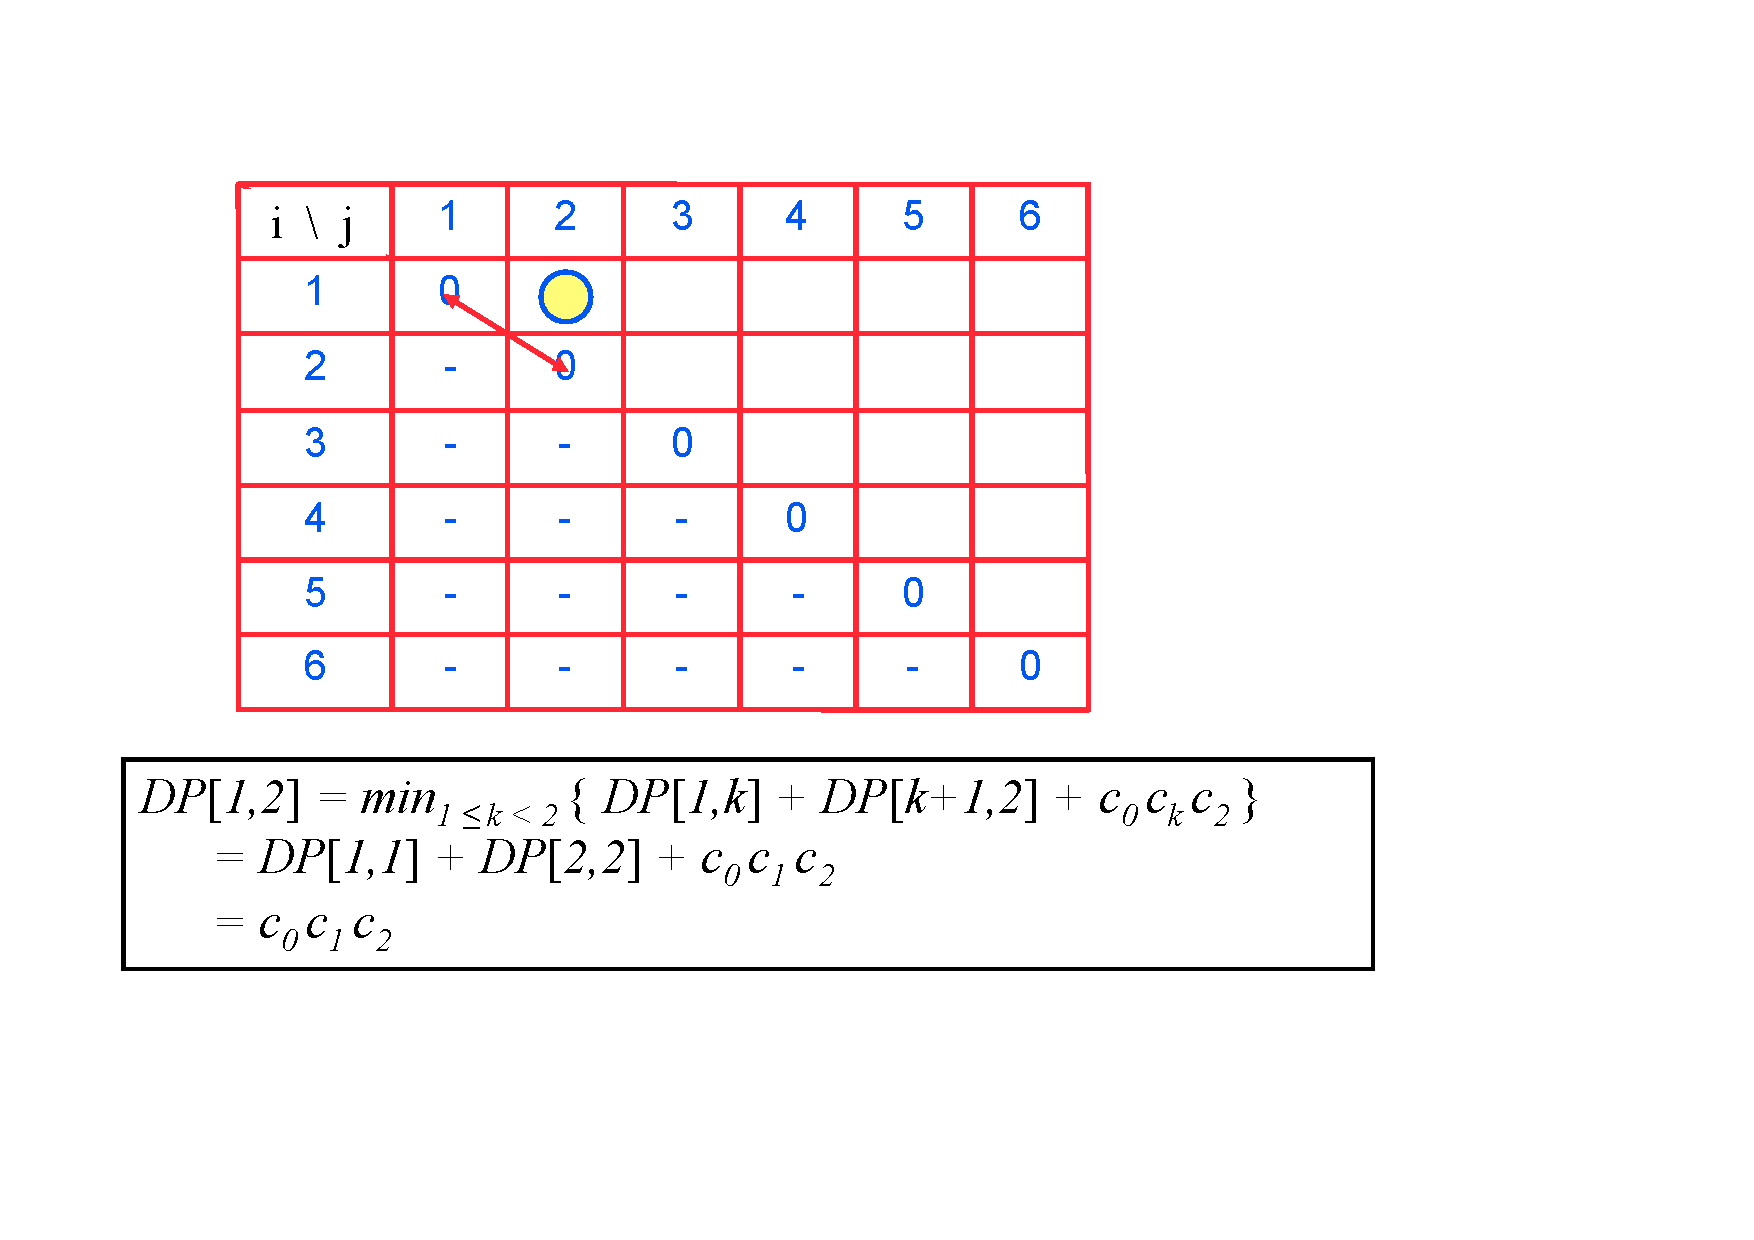
\includegraphics[width=9cm,page=1]{moltmatrici.pdf}
\end{center}
\end{frame}

%-------------------------------------------------------------------------
\begin{frame}{Esempio}
\vspace{-12pt}
\begin{center}
\includegraphics[width=9cm,page=2]{moltmatrici.pdf}
\end{center}
\end{frame}

%-------------------------------------------------------------------------
\begin{frame}{Esempio}
\vspace{-12pt}
\begin{center}
\includegraphics[width=9cm,page=3]{moltmatrici.pdf}
\end{center}
\end{frame}

%-------------------------------------------------------------------------
\begin{frame}{Esempio}
\vspace{-12pt}
\begin{center}
\includegraphics[width=9cm,page=4]{moltmatrici.pdf}
\end{center}
\end{frame}

%-------------------------------------------------------------------------
\begin{frame}{Esempio}
\vspace{-12pt}
\begin{center}
\includegraphics[width=9cm,page=5]{moltmatrici.pdf}
\end{center}
\end{frame}

%-------------------------------------------------------------------------
\begin{frame}{Dalla formula al codice}

\vspace{-9pt}
\begin{myboxtitle}[Input]
\BIL
\item Un vettore $c[0 \ldots n]$ contenente le dimensioni delle matrici
\BI
\item $c[0]$ è il numero di righe della prima matrice
\item $c[i-1]$ è il numero di righe della matrice $A_i$
\item $c[i]$ è il numero di colonne della matrice $A_i$
\EI
\item Due indici $i$, $j$ che rappresentano l'intervallo di matrici da moltiplicare
\EIL
\end{myboxtitle}

\begin{myboxtitle}[Output]
Il numero di moltiplicazioni scalari per calcolare il prodotto delle matrici comprese fra gli indici $i$ e $j$
\end{myboxtitle}

\end{frame}

%-------------------------------------------------------------------------
\begin{frame}{Approccio ricorsivo}

\vspace{-9pt}
\begin{Procedure}
\caption[A]{\INTEGER \fontproc{recPar}($\INTEGER[\,]\ c$, \INTEGER $i$, \INTEGER $j$)}
\eIf{$i=j$}
{ \Return\ $0$\; }
{
  $\Min = +\infty$\;
  \For{\INTEGER $k = i$ \TO\ $j-1$}{
    \INTEGER $q = \fontproc{recPar}(c, i, k) +  \fontproc{recPar}(c, k+1, j) + c[i-1] \cdot c[k] \cdot c[j]$\;
    \If{$q < \Min$}{$\Min = q$\;}
  }
  \Return \Min\;
}
\end{Procedure}

\BB{Complessità?}

\end{frame}

%-------------------------------------------------------------------------
\begin{frame}{Valutazione}

\vspace{-9pt}
\BB{Alcune riflessioni}
\BIL
\item La soluzione ricorsiva top-down è $\Omega(2^n$)
\item Non è poi migliore dell'approccio basato su forza bruta!
\item Il problema è che molti sottoproblemi vengono risolti più volte
\item Il numero di sottoproblemi è $\frac{n(n+1)}{2}$
\EIL

\end{frame}

%-------------------------------------------------------------------------
\begin{frame}{Versione bottom-up}

\vspace{-9pt}
\begin{myboxtitle}[Tabelle programmazione dinamica]
Due matrici $DP$, $\mathit{last}$ di dimensione $n \times n$ tali che:
\BIL
\item $DP[i][j]$ contiene il numero di moltiplicazioni scalari necessarie
per moltiplicare le matrici $A[i \ldots j]$
\item $\mathit{last}[i][j]$ contiene il valore $k$ dell'ultimo prodotto che minimizza il costo per il sottoproblema
\EIL
\end{myboxtitle}
\end{frame}

%-------------------------------------------------------------------------
\begin{frame}[shrink=10]{Versione bottom-up}

\vspace{-9pt}
\begin{Procedure}
\caption[A]{\textsf{computePar}($\INTARRAY\ c$, \INTEGER $n$)}	
$\INTARRAY[\,]\ DP = \NEW\ \INTEGER[1 \ldots n][1 \ldots n]$\;
$\INTARRAY[\,]\ \mathit{last} = \NEW\ \INTEGER[1 \ldots n][1 \ldots n]$\;
\For(\Comment*[f]{Fill main diagonal}){$i = 1$ \TO $n$}{$DP[i][i] = 0$\;}
\For(\Comment*[f]{$h$: diagonal index}){$h = 2$ \TO $n$}
{
  \For(\Comment*[f]{$i$: row}){$i = 1$ \TO\ $n-h+1$}
  {
    \INTEGER $j = i+h-1$\Comment*{$j$: column}
    $DP[i][j] = +\infty$\;
    \For(\Comment*[f]{$k$: last product}){$k = i$ \TO\ $j-1$} 
    {
      \INTEGER\ $\mathit{temp} = DP[i][k] + DP[k+1][j] + c[i-1] \cdot c[k] \cdot c[j]$\;
      \If{$\mathit{temp} < DP[i][j]$} 
      {
        $DP[i][j] = \mathit{temp}$\;
        $\mathit{last}[i][j] = k$\;
      }
    }
  }
}
\Return $DP[1][n]$\;
\end{Procedure}

\end{frame}


%-------------------------------------------------------------------------
\begin{frame}{}

\begingroup
\renewcommand*{\arraystretch}{1.0}
\vspace{-6pt}
\begin{columns}[T]
\column{0.68\textwidth}
\begin{tabular}{|r|r|r|r|r|r|r|}
\hline
$DP$ &  \textbf{1} & \textbf{2} & \textbf{3} & \textbf{4} & \textbf{5} & \textbf{6} \\\hline
\textbf{1} & \phantom{0}0 & \color{blue}{224} & \color{blue}{176} & \alert{218} & 276 & 350 \\\hline
\textbf{2} &   & 0 & 64 & \color{blue}{112} & 174 & 250 \\\hline
\textbf{3} &   &   & 0 & \color{blue}{24}    & 70 & 138 \\\hline
\textbf{4} &   &   &   & 0 & 30 & 90 \\\hline
\textbf{5} &   &   &   &   & 0 & 90 \\\hline
\textbf{6} &   &   &   &   &   & 0 \\\hline
\end{tabular}
\column{0.28\textwidth}
\begin{tabular}{|c|c|}
\hline
$i$ & $c[i]$ \\\hline
0 & 7 \\\hline
1 & 8 \\\hline
2 & 4 \\\hline
3 & 2 \\\hline
4 & 3 \\\hline
5 & 5 \\\hline
6 & 6 \\\hline
\end{tabular}
\end{columns}

\medskip
\setlength{\tabcolsep}{3pt}
\begin{tabular}{lllllllllllllllll}
$DP[1][4]$ & $=$ & $\displaystyle\min_{1 \leq k < 4}$ & \{ & $DP[1][k]$ & $+$ & $DP[k+1][4]$ & $+$ & $c_0 \cdot c_k \cdot c_4$ ~\} \\
        & $=$      & $\min$ & \{ & $DP[1][1]$ & $+$ & $DP[2][4]$ & $+$ & $c_0 \cdot c_1 \cdot c_4,$ \\
         &     &        & \{ & $DP[1][2]$ & $+$ & $DP[3][4]$ & $+$ & $c_0 \cdot c_2 \cdot c_4,$ \\
         &     &        & \{ & $DP[1][3]$ & $+$ & $DP[4][4]$ & $+$ & $c_0 \cdot c_3 \cdot c_4 ~\}$ \\
         &  $=$   & $\min$ & \{ & 0 & $+$ & 112 & $+$ & $7 \cdot 8 \cdot 3,$ \\
          &    &        & \{ & 224  & $+$ & 24 & $+$ & $7 \cdot 4 \cdot 3,$ \\
          &    &        & \{ & 176 & $+$ & 0 & $+$ & $7 \cdot 2 \cdot 3 ~\}$ \\
         &  $=$   & $\min$ & \{ & 280 & $,$ & 332 & $,$ & \alert{218} ~ \} \\
\end{tabular}
\endgroup

\end{frame}


%-------------------------------------------------------------------------
\begin{frame}{}

\begingroup
\renewcommand*{\arraystretch}{1.0}
\vspace{-6pt}
\begin{columns}[T]
\column{0.68\textwidth}
\begin{tabular}{|r|r|r|r|r|r|r|}
\hline
$\mathit{last}$ &  \textbf{1} & \textbf{2} & \textbf{3} & \textbf{4} & \textbf{5} & \textbf{6} \\\hline
\textbf{1} & \phantom{0}0 & \phantom{0}1 & \phantom{0}1 & \phantom{0}\alert{3} & \phantom{0}3 & \phantom{0}3 \\\hline
\textbf{2} &   & 0 & 2 & 3 & 3 & 3 \\\hline
\textbf{3} &   &   & 0 & 3 & 3 & 3 \\\hline
\textbf{4} &   &   &   & 0 & 4 & 5 \\\hline
\textbf{5} &   &   &   &   & 0 & 5 \\\hline
\textbf{6} &   &   &   &   &   & 0 \\\hline
\end{tabular}
\column{0.28\textwidth}
\begin{tabular}{|c|c|}
\hline
$i$ & $c[i]$ \\\hline
0 & 7 \\\hline
1 & 8 \\\hline
2 & 4 \\\hline
3 & 2 \\\hline
4 & 3 \\\hline
5 & 5 \\\hline
6 & 6 \\\hline
\end{tabular}
\end{columns}

\medskip
\setlength{\tabcolsep}{3pt}
\begin{tabular}{lllllllllllllllll}
$DP[1][4]$ & $=$ & $\displaystyle\min_{1 \leq k < 4}$ & \{ & $DP[1][k]$ & $+$ & $DP[k+1][4]$ & $+$ & $c_0 \cdot c_k \cdot c_4$ ~\} \\
        & $=$      & $\min$ & \{ & $DP[1][1]$ & $+$ & $DP[2][4]$ & $+$ & $c_0 \cdot c_1 \cdot c_4,$ \\
         &     &        & \{ & $DP[1][2]$ & $+$ & $DP[3][4]$ & $+$ & $c_0 \cdot c_2 \cdot c_4,$ \\
         &     &        & \{ & $DP[1][3]$ & $+$ & $DP[4][4]$ & $+$ & $c_0 \cdot c_3 \cdot c_4 ~\}$ \\
         &  $=$   & $\min$ & \{ & 0 & $+$ & 112 & $+$ & $7 \cdot 8 \cdot 3,$ \\
          &    &        & \{ & 224  & $+$ & 24 & $+$ & $7 \cdot 4 \cdot 3,$ \\
          &    &        & \{ & 176 & $+$ & 0 & $+$ & $7 \cdot 2 \cdot 3 ~\}$ \\
         &  $=$   & $\min$ & \{ & 280 & $,$ & 332 & $,$ & \alert{218} ~ \} \\
\end{tabular}
\endgroup

\end{frame}



%-------------------------------------------------------------------------
\begin{frame}{Parentesizzazione ottima}

\vspace{-9pt}
\begin{myboxtitle}[Considerazioni]
\BIL
\item Il costo computazionale è $O(n^3)$, in quanto ogni cella richiede $O(n)$ per essere riempita
\item Il costo della funzione si trova nella posizione $DP[1][n]$
\item E' anche necessario mostrare la soluzione trovata
\item Per questo motivo abbiamo registrato informazioni sulla soluzione nella matrice $\mathit{last}$
\EIL
\end{myboxtitle}

\end{frame}

%-------------------------------------------------------------------------
\begin{frame}{Ricostruzione della soluzione -- Stampa}

\vspace{-9pt}
\begin{Procedure}
\caption[A]{\textsf{computePar}($\INTARRAY\ c$, \INTEGER $n$)}	
[\ldots]\;
$\fontproc{printPar}(\mathit{last}, 1, n)$\;
\end{Procedure}


\begin{Procedure}
\caption[A]{\fontproc{printPar}($\INTARRAY[\,]\ \mathit{last}$, \INTEGER $i$, \INTEGER $j$)}
\eIf{$i \Eq j$}
{ \PRINT\ "A[";\ \PRINT\ $i$;\ \PRINT\ "]"\; }
{
  \PRINT\ "("; 
  $\printpar(\mathit{last}, i, \mathit{last}[i][j])$; 
  \PRINT\ "$\cdot$"; 
  $\printpar(\mathit{last}, \mathit{last}[i][j]+1, j)$; 
  \PRINT\ ")"\;
}
\end{Procedure}

\end{frame}

%-------------------------------------------------------------------------
\begin{frame}{Ricostruzione della soluzione -- Calcolo effettivo}

\vspace{-9pt}
\begin{Procedure}
\caption[A]{$\INTARRAY[\,]$ \fontproc{multiply}($\mathbf{matrix}[\,]\ A$, $\INTARRAY[\,]\ S$, \INTEGER $i$, \INTEGER $j$)}
\eIf{$i \Eq j$}
{ \Return\ $A[i]$\; }
{
  $\INTARRAY[\,]\ X = \fontproc{multiply}(\mathit{last}, i, \mathit{last}[i][j])$\;
  $\INTARRAY[\,]\ Y = \fontproc{multiply}(\mathit{last}, \mathit{last}[i][j]+1, j)$\;
  \Return\ $\fontproc{matrix-multiplication}(X,Y)$\;
}
\end{Procedure}

\end{frame}

%-------------------------------------------------------------------------
\begin{frame}{Esempio}

\vspace{-9pt}
\begin{columns}[T]
\column{0.45\textwidth}
\begin{align*}
A[1 \ldots 6] &= A[1 \ldots 3] \cdot A[4 \ldots 6] \\
A[1 \ldots 3] &= A_1 \cdot A[2 \ldots 3]\\
A[4 \ldots 6] &= A[4 \ldots 5] \cdot A_6\\
A[2 \ldots 3] &= A_2 \cdot A_3 \\
A[4 \ldots 5] &= A_4 \cdot A_5
\end{align*}

\column{0.50\textwidth}
\begin{tabular}{|c|c|c|c|c|c|c|}
\hline
$\mathit{last}$ &  \textbf{1} & \textbf{2} & \textbf{3} & \textbf{4} & \textbf{5} & \textbf{6} \\\hline
\textbf{1} & 0 & 1 & 1 & 3 & 3 & 3 \\\hline
\textbf{2} &   & 0 & 2 & 3 & 3 & 3 \\\hline
\textbf{3} &   &   & 0 & 3 & 3 & 3 \\\hline
\textbf{4} &   &   &   & 0 & 4 & 5 \\\hline
\textbf{5} &   &   &   &   & 0 & 5 \\\hline
\textbf{6} &   &   &   &   &   & 0 \\\hline
\end{tabular}
\end{columns}

\begin{myboxtitle}[Risultato finale]
\[
 A = ( ( A_1 \cdot  (A_2 \cdot A_3) ) \cdot ( (A_4 \cdot A_5 )  \cdot A_6) )
\]
\end{myboxtitle}

\end{frame}

%-------------------------------------------------------------------------
\begin{frame}{Prodotto di catena di matrici}

\vspace{-9pt}
\begin{myboxtitle}[Take-home message -- prendi e porta a casa]
A volte, bisogna fare attenzione a come riempire la tabella - non è detto che 
riempire una riga dopo l'altra sia possibile.
\end{myboxtitle}

\end{frame}

%%%%%%%%%%%%%%%%%%%%%%%%%%%%%%%%%%%%%%%%%%%%%%%%%%%%%%%%%%%%%%%%%%%%%%%%%%%%%
\section{Insieme indipendente di intervalli pesati}
%%%%%%%%%%%%%%%%%%%%%%%%%%%%%%%%%%%%%%%%%%%%%%%%%%%%%%%%%%%%%%%%%%%%%%%%%%%%%

%-------------------------------------------------------------------------
\begin{frame}{Insieme indipendente di intervalli pesati -- Introduzione}

\vspace{-9pt}
\begin{myboxtitle}[Input]
Siano dati $n$ intervalli distinti $[a_1, b_1[, \ldots, [a_n,b_n[$ della retta reale, aperti a destra, dove all'intervallo $i$ è associato un profitto $w_i, 1 \leq i \leq n$. 
\end{myboxtitle}

\begin{myboxtitle}[Intervalli disgiunti]
Due intervalli $i$ e $j$ si dicono \alert{disgiunti} se:  $b_j \leq a_i$  oppure  $b_i \leq a_j$
\end{myboxtitle}

\begin{myboxtitle}[Problema]
Trovare un \alert{insieme indipendente di peso massimo}, ovvero un sottoinsieme di intervalli disgiunti tra loro tale che la somma dei loro profitti sia la più
grande possibile.
\BI
\item Esempio: prenotazione di una sala conferenza
\EI
\end{myboxtitle}

\end{frame}

%-------------------------------------------------------------------------
\begin{frame}{Esempio}

\vspace{-12pt}
\begin{center}
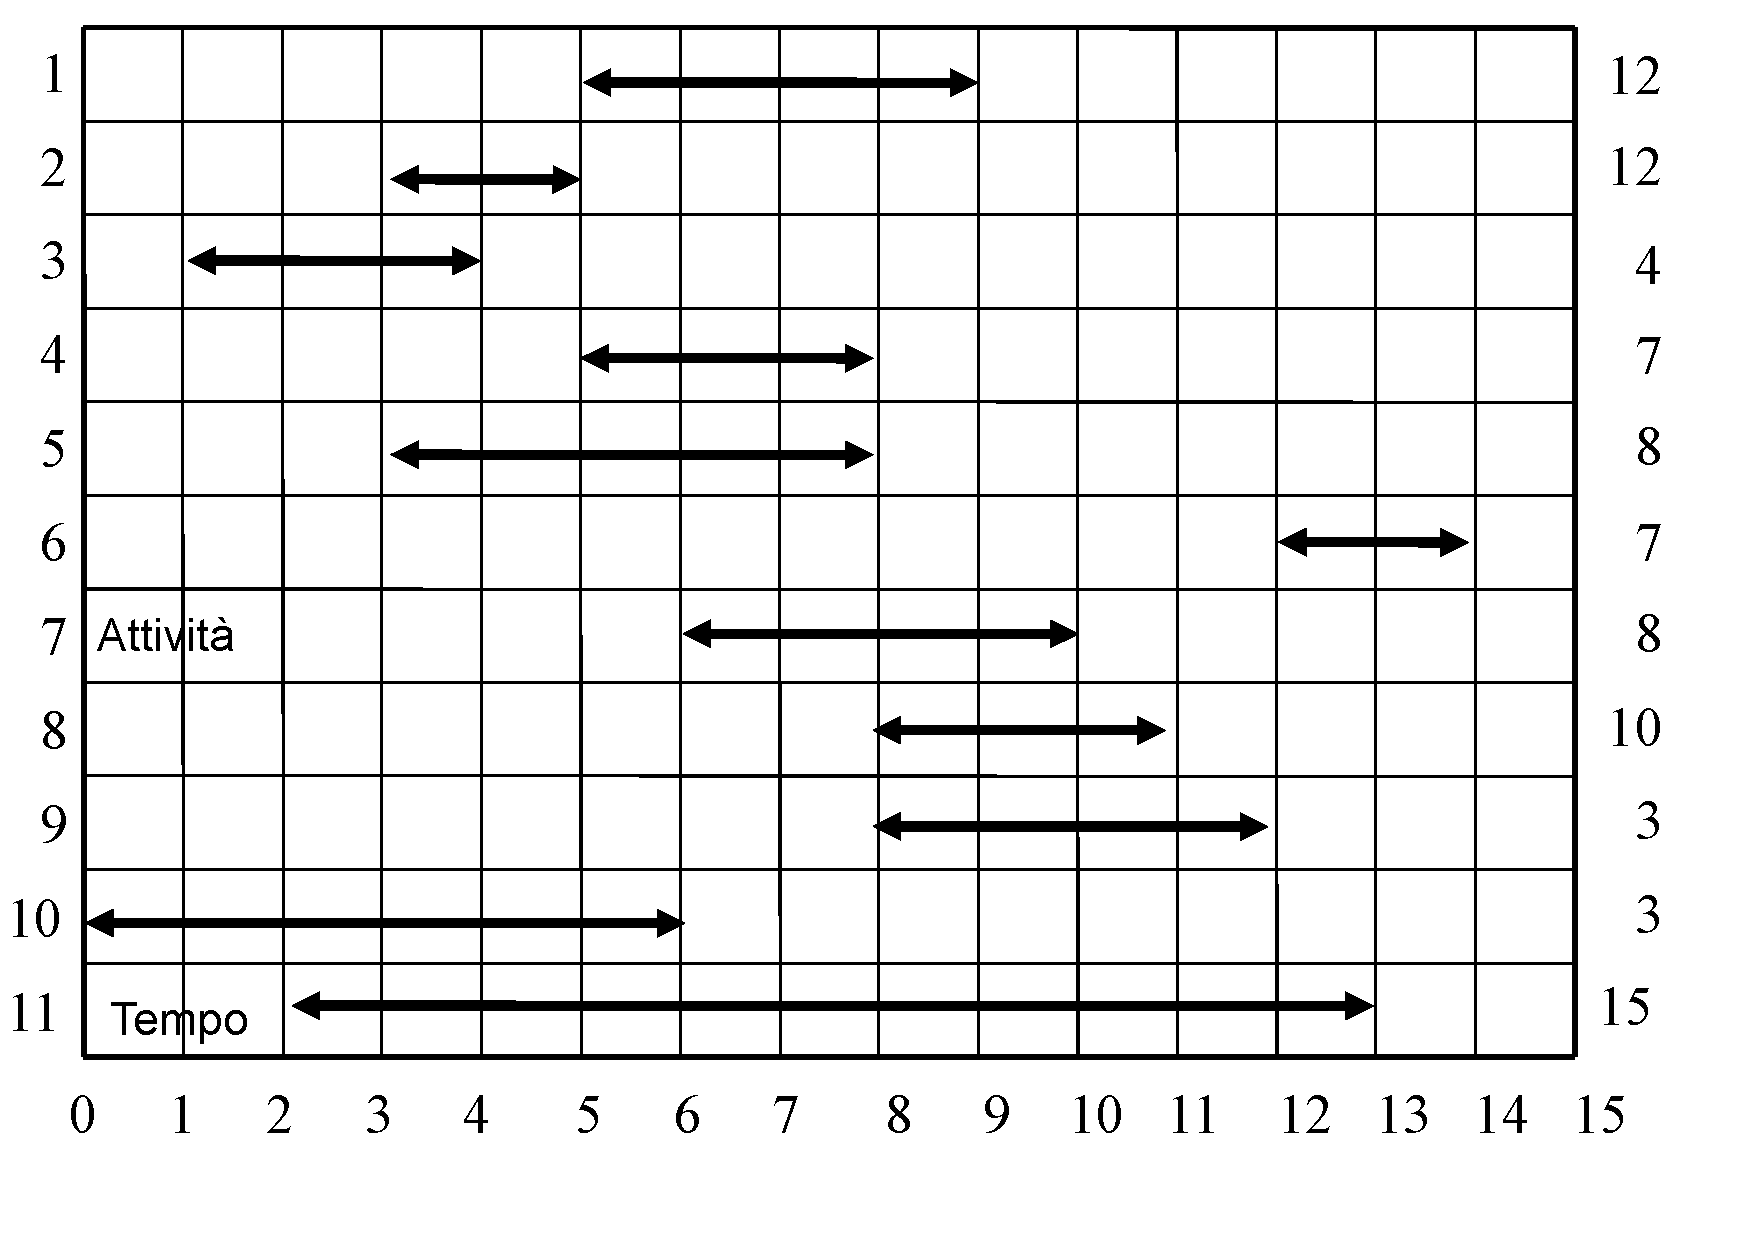
\includegraphics[width=0.95\textwidth,page=1]{intervalli-esempio.pdf}
\end{center}

\end{frame}

%-------------------------------------------------------------------------
\begin{frame}{Esempio}

\vspace{-12pt}
\begin{center}
\includegraphics[width=0.95\textwidth,page=2]{intervalli-esempio.pdf}
\end{center}

\end{frame}

%-------------------------------------------------------------------------
\begin{frame}{Pre-elaborazione}

\vspace{-9pt}
Per usare la programmazione dinamica, è necessario effettuare una pre-elaborazione: ordinare gli intervalli per estremi finali crescenti

  \[
     b_1 \leq b_2 \leq \ldots \leq b_n
  \]

\BB{Profitto massimo, prima versione}
$DP[i]$ contiene il profitto massimo ottenibile con i primi $i$ intervalli

\[
  DP[i] = \begin{cases}
    0 & i = 0 \\
    \max (DP[i-1], \max \{ DP[j]+w_i : j < i \wedge b_j \leq a_i \} ) & i > 0
  \end{cases}
\]

\BB{Costo computazionale dell'algoritmo associato a questa formula?}
\pause 

\smallskip
$O(n^2)$

\end{frame}

%-------------------------------------------------------------------------
\begin{frame}{Pre-elaborazione}

\vspace{-9pt}
Una seconda possibile pre-elaborazione consiste nel pre-calcolare il \alert{predecessore} \alert{$\mathit{pred}_i = j$} di $i$, dove:
\BIL
\item $j<i$ è il massimo indice tale che $b_j \leq a_i$
\item se non esiste tale indice, $\mathit{pred}_i=0$.
\EIL

\begin{center}
\IG{0.6}{predecessore.pdf}
\end{center}

\BB{Profitto massimo, seconda versione}

\[
  DP[i] = \begin{cases}
    0 & i = 0 \\
    \max (DP[i-1], DP[\mathit{pred}_i] + w_i) & i > 0
  \end{cases}
\]

\end{frame}

%-------------------------------------------------------------------------
\begin{frame}{Pre-elaborazione - calcolo predecessori}

\vspace{-9pt}
\begin{Procedure}
\caption[A]{$\INTEGER[\,]$ \textsf{computePredecessor($\INTEGER[\,]\ a$, $\INTEGER[\,]\ a$, \INTEGER $n$)}}    
$\INTARRAY\ \mathit{pred} = \NEW\ \INTEGER[0 \ldots n]$\;
$\mathit{pred}[0] = 0$\;
\For{$i = 1$ \TO $n$}{
  $j = i - 1$\;
  \While{$j > 0$ \AND\ $b[j] > a[i]$}{
    $j = j-1$\;
  }
  $\mathit{pred}[i] = j$\;
}
\Return $\mathit{pred}$\;
\end{Procedure}

\vspace{-9pt}
\begin{columns}[T]
\column{0.65\textwidth}
\BB{Quanto costa pre-calcolare i predecessori?}
\pause
\column{0.25\textwidth}
\bigskip\smallskip
$O(n^2)$
\end{columns}

\begin{columns}[T]
\column{0.65\textwidth}
\BB{Si può fare meglio di così?}
\pause
\column{0.25\textwidth}
\bigskip\smallskip
Sì!
\end{columns}

\end{frame}

%-------------------------------------------------------------------------
\begin{frame}[shrink=10]{Versione completa}

\vspace{-9pt}
\begin{Procedure}
\caption[A]{\Set\ \maxinterval($\INTARRAY\ a,\ \INTARRAY\ b,\ \INTARRAY w$, \INTEGER $n$)}	

\{ ordina gli intervalli per estremi di fine crescenti \}\;
$\INTARRAY\ pred = \textsf{computePredecessor}(a,b,n)$\;
$\INTARRAY\ DP = \NEW\ \INTEGER[0 \mldots n]$\;
$DP[0] = 0$\;
\For{$i = 1$ \TO\ $n$}
{
  $DP[i] = \MAX(DP[i-1], w[i] + DP[\mathit{pred}[i]])$\;
}
$i = n$\;
$\Set\ S = \setconstructor()$\;
\While{$i>0$}
{
  \eIf{$DP[i-1]> w[i] + DP[\mathit{pred}[i]]$}{
    $i = i-1$\;
  }{
    $S.\setinsert(i)$\;
    $i = \mathit{pred}[i]$\;
  }
}
\Return $S$\;
\end{Procedure}

\end{frame}

%-------------------------------------------------------------------------
\begin{frame}{Costo computazionale}

\vspace{-9pt}
\BB{Costo computazionale}
\BIL
\item Ordinamento intervalli: \alert{$O(n \log n)$}
\item Calcolo predecessori: \alert{$O(n \log n)$}
\item Riempimento tabella $DP$: \alert{$O(n)$}
\item Ricostruzione soluzione: \alert{$O(n)$}
\item Algoritmo totale: \alert{$O(n \log n)$}
\EIL

\BB{Esercizio}
Scrivere una funzione di calcolo predecessori in tempo $O(n \log n)$

\end{frame}

%-------------------------------------------------------------------------
\begin{frame}{Insieme indipendente di intervalli pesati -- Conclusioni}

\vspace{-9pt}
\begin{myboxtitle}[Take-home message -- prendi e porta a casa]
Talvolta, può essere necessario pre-processare l'input per poter applicare nella maniera più efficiente possibile la programmazione dinamica
\end{myboxtitle}

\end{frame}

%-------------------------------------------------------------------------
\begin{frame}{Per concludere}

\vspace{-9pt}
\begin{myboxtitle}[Una lezione ancora più importante]
La programmazione dinamica non è la soluzione di tutti i vostri problemi. Esistono altre tecniche che possono fare "meglio di così". Inoltre, è possibile che soluzioni ad-hoc possano essere migliori
\end{myboxtitle}

\begin{myboxtitle}[Esempi]
\BIL
\item \alert{Longest increasing subsequence}: può essere risolto in tempo $O(n \log n)$
\item \alert{Longest common subsequence}: può essere risolto in tempo $O(mn/\log n)$ (con alfabeto limitato)
\item \alert{Four Russians algorithm}: tecnica generale che può essere applicata a vari problemi su matrice con alfabeto limitato $O(n^2/\log n)$
\BI
\item Edit distance
\item Transitive closure
\item ...
\EI
\EIL
\end{myboxtitle}

\end{frame}

%-------------------------------------------------------------------------
\begin{frame}{Approccio generale}

\vspace{-9pt}
\IG{1.0}{progrdyn.pdf}

\end{frame}

%-------------------------------------------------------------------------
\begin{frame}{Risolvere problemi con programmazione dinamica}

\vspace{-9pt}
\begin{myboxtitle}[Fasi]
\BIL 
\item Caratterizzare la \alert{struttura} di una soluzione ottima
\item Definire ricorsivamente il \alert{valore} di una soluzione ottima
\item Calcolare il \alert{valore} di una soluzione ottima "bottom-up" (dal basso verso l'alto)
\item Ricostruzione di una soluzione ottima 
\EIL
\end{myboxtitle}

\end{frame}

\end{document}


